\section{Desenvolvimento}

Esta seção apresenta a solução proposta neste trabalho e detalha os elementos
técnicos que sustentam a sua concepção. Aqui são abordados os requisitos
funcionais e não funcionais que foram levantados, a arquitetura do sistema, a
modelagem do banco de dados em terceira forma normal e os diagramas que ajudam a
mostrar como a plataforma funciona, como ela é estruturada por dentro e como
fica a sua infraestrutura.

\subsection{Requisitos do Sistema}

Para que o desenvolvimento seguisse uma direção bem definida, foram levantados
os requisitos funcionais e não funcionais do sistema. Os requisitos funcionais
descrevem o que se espera que a plataforma faça do ponto de vista do usuário,
enquanto os não funcionais tratam de aspectos como segurança, desempenho,
disponibilidade e escalabilidade, que não aparecem direto para quem usa, mas
que sustentam o sistema por trás. A Tabela \ref{tab-requisitos} traz os
principais requisitos funcionais separados por módulo.

\begin{table}[!ht]
\centering
\caption{Principais requisitos funcionais da plataforma.}
\label{tab-requisitos}
\scriptsize
\begin{tabular}{|l|l|l|}
\hline
\textbf{Código} & \textbf{Módulo} & \textbf{Descrição} \\
\hline
RF-AUT-001 & Autenticação & Login via CPF e senha \\
\hline
RF-AUT-003 & Autenticação & Recuperação de senha por e-mail \\
\hline
RF-AUT-007 & Autenticação & Ativação de conta por código \\
\hline
RF-FOR-001 & Fórum & Criar tópico vinculado a disciplina \\
\hline
RF-FOR-003 & Fórum & Responder tópicos \\
\hline
RF-FOR-009 & Fórum & Votar em respostas \\
\hline
RF-FOR-010 & Fórum & Marcar melhor resposta \\
\hline
RF-FOR-013 & Fórum & Restringir publicação por decisão pedagógica \\
\hline
RF-FOR-015 & Fórum & Busca semântica e textual nos tópicos \\
\hline
RF-FOR-018 & Fórum & Analisar denúncia com justificativa ao autor \\
\hline
RF-COL-001 & Colaboração & Propor trabalho em grupo com material de apoio \\
\hline
RF-COL-004 & Colaboração & Formar grupos por escolha ou sorteio \\
\hline
RF-COL-007 & Colaboração & Conversa privada por grupo, em tempo real \\
\hline
RF-COL-011 & Colaboração & Encaminhar dúvida do grupo à monitoria \\
\hline
RF-VOL-001 & Voluntariado & Cadastrar oportunidade \\
\hline
RF-VOL-003 & Voluntariado & Inscrição em oportunidade \\
\hline
RF-VOL-007 & Voluntariado & Emissão de certificado em PDF \\
\hline
RF-PRF-002 & Perfil & Editar perfil com imagem e biografia \\
\hline
RF-PRF-006 & Perfil & Acompanhar o próprio percurso por disciplina \\
\hline
RF-NOT-001 & Notificações & Notificações em tempo real \\
\hline
\end{tabular}
\\ \vspace{4pt}
\textit{\scriptsize Fonte: Elaborado pela autora (2026).}
\end{table}

Cada requisito possui a sua descrição funcional e técnica, a indicação do ator
responsável por usá-lo e o nível de prioridade, parâmetros que ajudam a definir
a ordem em que as funcionalidades vão sendo implementadas ao longo do projeto.

Ao longo do desenvolvimento, dois conjuntos de requisitos foram revistos. O
sistema de reputação e o ranking semestral, previstos inicialmente para
incentivar a participação, foram removidos do escopo. A decisão partiu da
constatação de que a pontuação pública desloca o incentivo de ajudar para o de
pontuar, e de que esse deslocamento é mais visível em um fórum de disciplina,
no qual as mesmas pessoas convivem ao longo de todo o semestre, do que em uma
comunidade aberta e numerosa. O reconhecimento permaneceu apenas na marcação de
melhor resposta, que serve a quem consulta o tópico depois. Em contrapartida,
foi incorporado o módulo de colaboração, com trabalhos em grupo, conversa
privada por equipe e encaminhamento de dúvida à monitoria, respondendo a uma
lacuna identificada durante o levantamento: a discussão de trabalho em grupo
acontecia integralmente fora dos sistemas da universidade.

\subsection{Arquitetura do Sistema}

A arquitetura da plataforma foi pensada para separar as responsabilidades de
cada parte do sistema, como mostra a Figura \ref{fig-arquitetura}. O usuário
acessa a plataforma pelo navegador, que conversa com o frontend desenvolvido em
React.js com TypeScript e estilizado com o TailwindCSS. Esse frontend, por sua
vez, faz requisições HTTP à API REST do backend construído em Django com o
Django REST Framework, que é quem cuida da lógica de negócio, das validações e
das regras de acesso. O backend se conecta ao PostgreSQL para guardar os dados e
ao Redis para gerenciar os tokens JWT, os refresh tokens e as sessões que estão
ativas. Já para as funcionalidades que precisam de tempo real, como as
notificações e os chats, o navegador mantém uma conexão WebSocket direta com o
servidor de aplicação, gerenciada pelo Django Channels, o que permite enviar e
receber mensagens sem precisar ficar atualizando a página na mão.

A busca do fórum conta ainda com um componente opcional de recuperação
semântica, descrito na Subseção \ref{busca-semantica}, que utiliza a extensão
pgvector do PostgreSQL para armazenar representações vetoriais das publicações.

\begin{figure}[!ht]
\centering
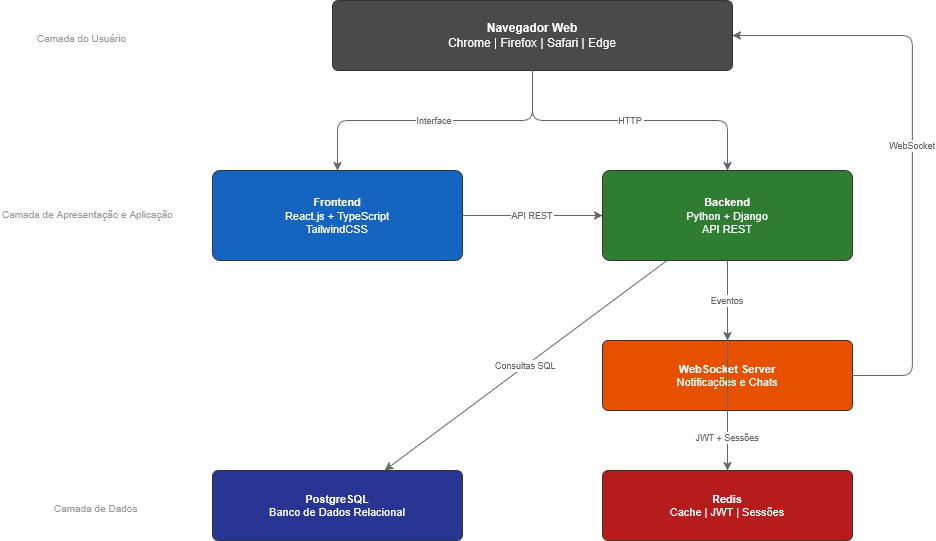
\includegraphics[width=\columnwidth]{figs/arquitetura.png}
\caption{Arquitetura do sistema proposto.}
\label{fig-arquitetura}
\textit{\scriptsize Fonte: Elaborado pela autora (2026).}
\end{figure}

Essa separação em camadas traz algumas vantagens para o sistema. Ela dá mais
modularidade, facilita a manutenção de cada parte de forma independente e ainda
permite que cada pedaço do sistema seja escalado conforme a demanda for
crescendo. Além disso, o fato de a camada de apresentação ficar separada da
camada de aplicação acaba abrindo caminho para uma evolução futura em direção a
aplicativos móveis nativos, já que a API REST construída pode ser consumida por
qualquer cliente compatível, e não só pelo frontend web.

\subsection{Modelagem do Banco de Dados}

A modelagem do banco de dados foi feita em terceira forma normal (3FN)
\citep{date2003}, o que ajuda a deixar as informações organizadas sem repetição
e com a integridade referencial preservada. O banco conta com 26 tabelas
espalhadas em seis módulos, como mostra a Tabela \ref{tab-banco}, agrupadas
de acordo com a funcionalidade que cada uma atende dentro do sistema.

\begin{table}[!ht]
\centering
\caption{Tabelas do banco de dados organizadas por módulo.}
\label{tab-banco}
\scriptsize
\begin{tabular}{|l|p{5.2cm}|}
\hline
\textbf{Módulo} & \textbf{Tabelas} \\
\hline
Autenticação & Usuario, CodigoAtivacao, RoleGlobal \\
\hline
Fórum & Curso, Disciplina, PermissaoDisciplina, Post, HistoricoEdicao, Voto, ReacaoPersiste, Arquivo, AlertaConteudo \\
\hline
Colaboração & Trabalho, ArquivoTrabalho, GrupoTrabalho, MembroGrupo, Conversa, ParticipanteConversa, MensagemChat, SolicitacaoAjuda \\
\hline
Voluntariado & Oportunidade, InscricaoVoluntariado, Certificado \\
\hline
Notificações e Auditoria & Notificacao, AuditLog \\
\hline
Busca & IndicePost \\
\hline
\end{tabular}
\\ \vspace{4pt}
\textit{\scriptsize Fonte: Elaborado pela autora (2026).}
\end{table}

A tabela Curso e os campos de período, carga horária, ementa, pré-requisitos e
co-requisitos em Disciplina permitem que a matriz curricular seja importada
diretamente do Projeto Pedagógico do Curso, em vez de cadastrada manualmente.
A oferta de cada semestre é derivada da paridade do período: disciplinas de
período ímpar são ofertadas no primeiro semestre e as de período par, no
segundo.

Vale registrar uma constatação da implementação. O PPC do curso de Ciência da
Computação declara o período de oferta de cada disciplina em dois pontos
distintos do documento, e eles divergem em quatro casos. A plataforma segue o
ementário, que organiza as disciplinas em grades por período e corresponde ao
desenho da oferta semestral efetivamente montada pela coordenação. A
divergência não seria percebida em uma leitura do documento, mas se torna
visível quando ele é traduzido em estrutura de dados, o que ilustra um efeito
secundário da informatização de normas acadêmicas: a implementação fiel expõe
inconsistências que o texto acomoda.

Durante a modelagem, foram tomadas algumas decisões pensando na segurança, na
auditabilidade e na manutenção do sistema. Todas as tabelas usam o UUID
(\textit{Universally Unique Identifier}) \citep{leach2005} como chave primária no
lugar dos identificadores sequenciais, uma escolha que dificulta a enumeração
dos recursos a partir das URLs e reduz o risco de expor dados internos sem
querer. As tabelas principais ainda contam com o campo \texttt{deleted\_at}, que
implementa a remoção lógica: em vez de apagar o registro, o sistema marca a data
em que ele deixou de valer, prática alinhada ao tratamento de dados orientados a
tempo descrito por \cite{snodgrass1999}. O conteúdo some da interface, mas
permanece recuperável em caso de exclusão indevida e disponível para auditoria.
Essa escolha convive com um limite: a Lei Geral de Proteção de Dados
\citep{brasil2018} assegura ao titular o direito à eliminação dos seus dados
pessoais, de modo que a remoção lógica não substitui a exclusão definitiva
quando ela for solicitada, e sim atende ao caso distinto da retirada de conteúdo
por moderação ou por engano do próprio autor.

O controle de acesso foi dividido em duas tabelas diferentes: a
PermissaoDisciplina, que cuida do papel do usuário dentro de cada disciplina
específica, permitindo que um mesmo aluno seja monitor em uma matéria e aluno em
outra, e a RoleGlobal, que fica com os papéis institucionais, como o de
administrador e o de organização, que não dependem de disciplina. Essa separação
coloca em prática o modelo de controle de acesso baseado em papéis (RBAC,
\textit{Role-Based Access Control}) \citep{sandhu1996} de um jeito mais
flexível, evitando que qualquer mudança no controle de acesso acabe mexendo na
tabela principal de usuários.

Sobre esse modelo, o sistema estabelece uma distinção que não se resolve apenas
com a hierarquia usual de papéis: a diferença entre supervisionar e participar.
A coordenação do curso responde por todas as disciplinas e precisa enxergá-las
por inteiro, mas não está matriculada em nenhuma turma e não leciona. Uma
implementação que trate o administrador como detentor de todas as permissões
faria com que a coordenação pudesse entrar em um grupo de trabalho, publicar
dúvida em uma disciplina que não cursa ou responder a um pedido de ajuda cujo
enunciado desconhece. A plataforma separa, portanto, dois predicados distintos:
um que autoriza a moderação de conteúdo, satisfeito também pelo administrador,
e outro que autoriza a condução da turma, que exige vínculo de professor ou
monitor com aquela disciplina específica. Organizar equipes, sortear grupos e
atender dúvidas de trabalho pressupõem conhecimento do enunciado, dos alunos e
do momento do conteúdo, e são atribuições de quem ministra a disciplina naquele
semestre.

A tabela AuditLog guarda todas as ações relevantes que acontecem no sistema,
registrando o endereço IP, o agente do navegador e o usuário responsável por
cada operação. Os registros dessa tabela não podem ser apagados em nenhuma
situação, o que garante a rastreabilidade que é necessária para fins de
segurança e de conformidade. Já os tokens de autenticação JWT (\textit{JSON Web
Token}) e os refresh tokens ficam guardados no Redis, e não no PostgreSQL, por
serem dados que mudam o tempo todo e que precisam de leitura e escrita rápidas,
algo em que um banco em memória acaba se saindo bem melhor que o banco
relacional.

\subsection{Diagrama Entidade-Relacionamento}

A Figura \ref{fig-er} mostra o diagrama entidade-relacionamento simplificado do
sistema, no qual as 26 tabelas aparecem agrupadas por módulo, com os seus
principais campos e os relacionamentos entre elas. Essa representação também foi
feita em terceira forma normal para evitar a repetição e garantir a integridade
dos dados que ficam guardados, mostrando de forma visual a mesma estrutura que
já foi descrita na Tabela \ref{tab-banco}.

\begin{figure}[H]
\centering
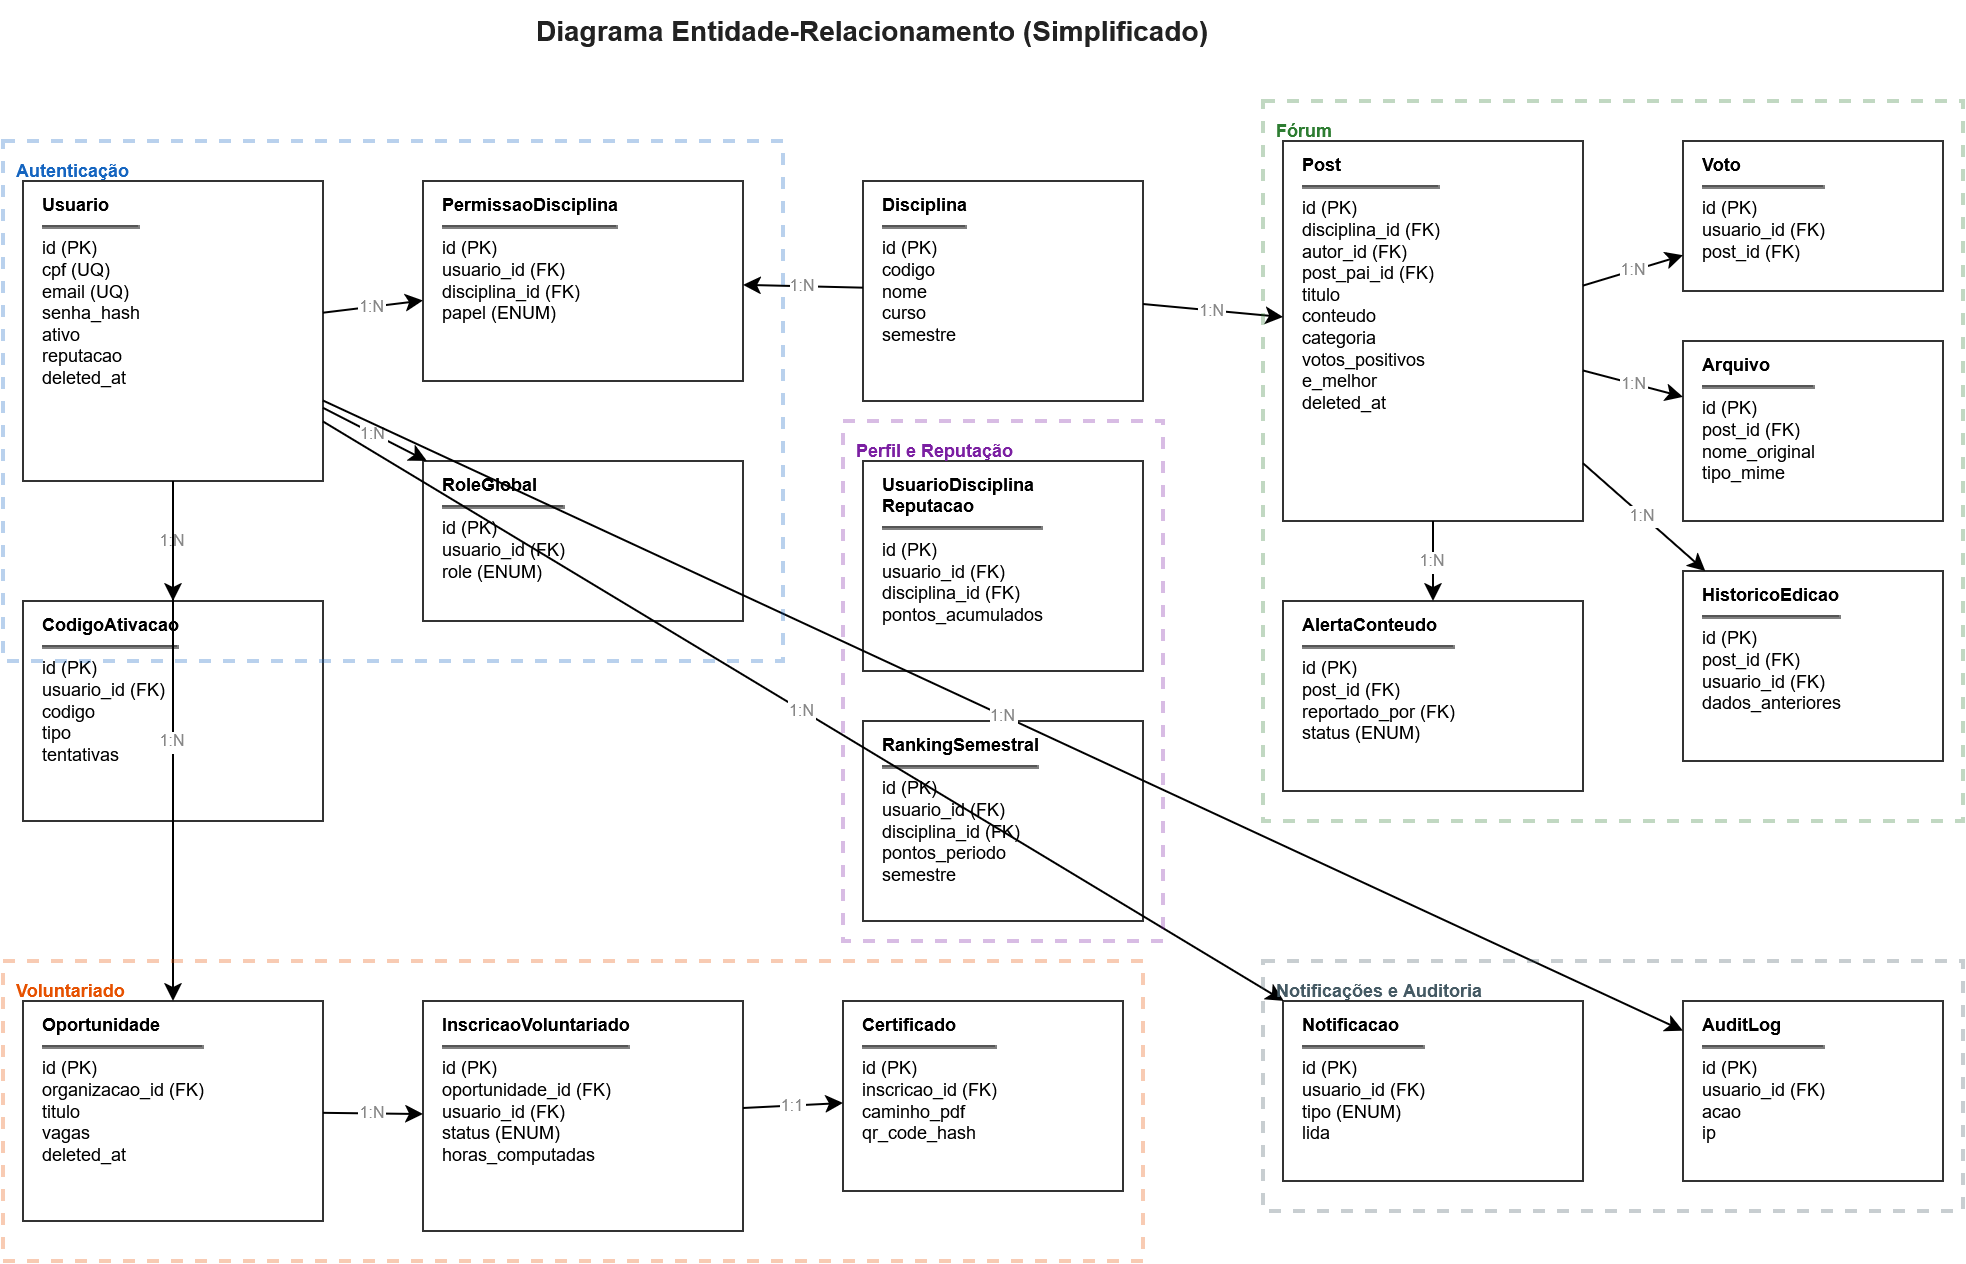
\includegraphics[width=0.50\textwidth]{figs/diagrama-er.png}
\caption{Diagrama entidade-relacionamento simplificado do sistema.}
\label{fig-er}
\textit{\scriptsize Fonte: Elaborado pela autora (2026).}
\end{figure}

\subsection{Recuperação Semântica de Publicações}
\label{busca-semantica}

Um fórum de disciplina acumula perguntas equivalentes formuladas com
vocabulários diferentes. As dúvidas ``por que meu laço executa uma vez a mais''
e ``erro de \textit{off-by-one} em vetor'' descrevem o mesmo problema e não
compartilham nenhum termo, de modo que a busca por palavra-chave jamais
relaciona uma à outra. O efeito prático é a republicação da mesma dúvida ao
longo dos semestres e a perda do conhecimento já registrado.

Para tratar esse caso, a plataforma incorpora um mecanismo de recuperação
semântica. Cada publicação é convertida em um vetor de 384 dimensões por um
modelo multilíngue de representação de sentenças \citep{reimers2019}, e esses
vetores são armazenados em uma tabela própria, indexada pela extensão pgvector
do PostgreSQL. A consulta do usuário passa pelo mesmo modelo, e a recuperação
ordena as publicações pela distância do cosseno em relação a ela, o que
aproxima textos por significado e não por coincidência de termos.

Três decisões de projeto orientaram essa implementação. A primeira é que os
vetores são gerados localmente, na própria infraestrutura, e não por serviço
externo: o conteúdo do fórum é material acadêmico de estudantes identificáveis,
e a transmissão desses textos a terceiros introduziria uma questão de
tratamento de dados pessoais desnecessária ao propósito do sistema. A segunda é
que o índice reside em tabela separada das publicações, de modo que a
substituição do modelo de representação implique uma reindexação isolada, e não
uma migração da estrutura do fórum. A terceira é que o recurso é opcional: na
ausência das bibliotecas correspondentes, a busca responde por correspondência
textual e nenhuma outra funcionalidade é afetada, o que evita que a
disponibilidade do fórum dependa de um componente acessório.

\subsection{Acessibilidade}

Por se tratar de sistema destinado a uma instituição federal de ensino, a
acessibilidade digital constitui obrigação legal, estabelecida pelo Decreto
n\textsuperscript{o} 5.296/2004 e pela Lei Brasileira de Inclusão
\citep{brasil2015}, e não recurso complementar. As diretrizes seguidas são as
da recomendação WCAG 2.1 \citep{w3c2018}, referência adotada pelo Modelo de
Acessibilidade em Governo Eletrônico brasileiro. A interface declara o idioma
português no elemento raiz do documento, condição para que leitores de tela
apliquem a pronúncia correta; mantém indicação visível de foco em todos os
elementos navegáveis por teclado; oferece atalho para o conteúdo principal como
primeiro elemento focalizável, evitando que a navegação percorra a barra lateral
a cada mudança de página; atribui rótulos acessíveis aos controles
representados apenas por ícone; e respeita a preferência do sistema operacional
por movimento reduzido. As combinações de cor foram verificadas quanto ao
contraste mínimo nos dois temas disponíveis.

\subsection{Casos de Uso}
\label{casos-de-uso}

\begin{figure}[!ht]
\centering
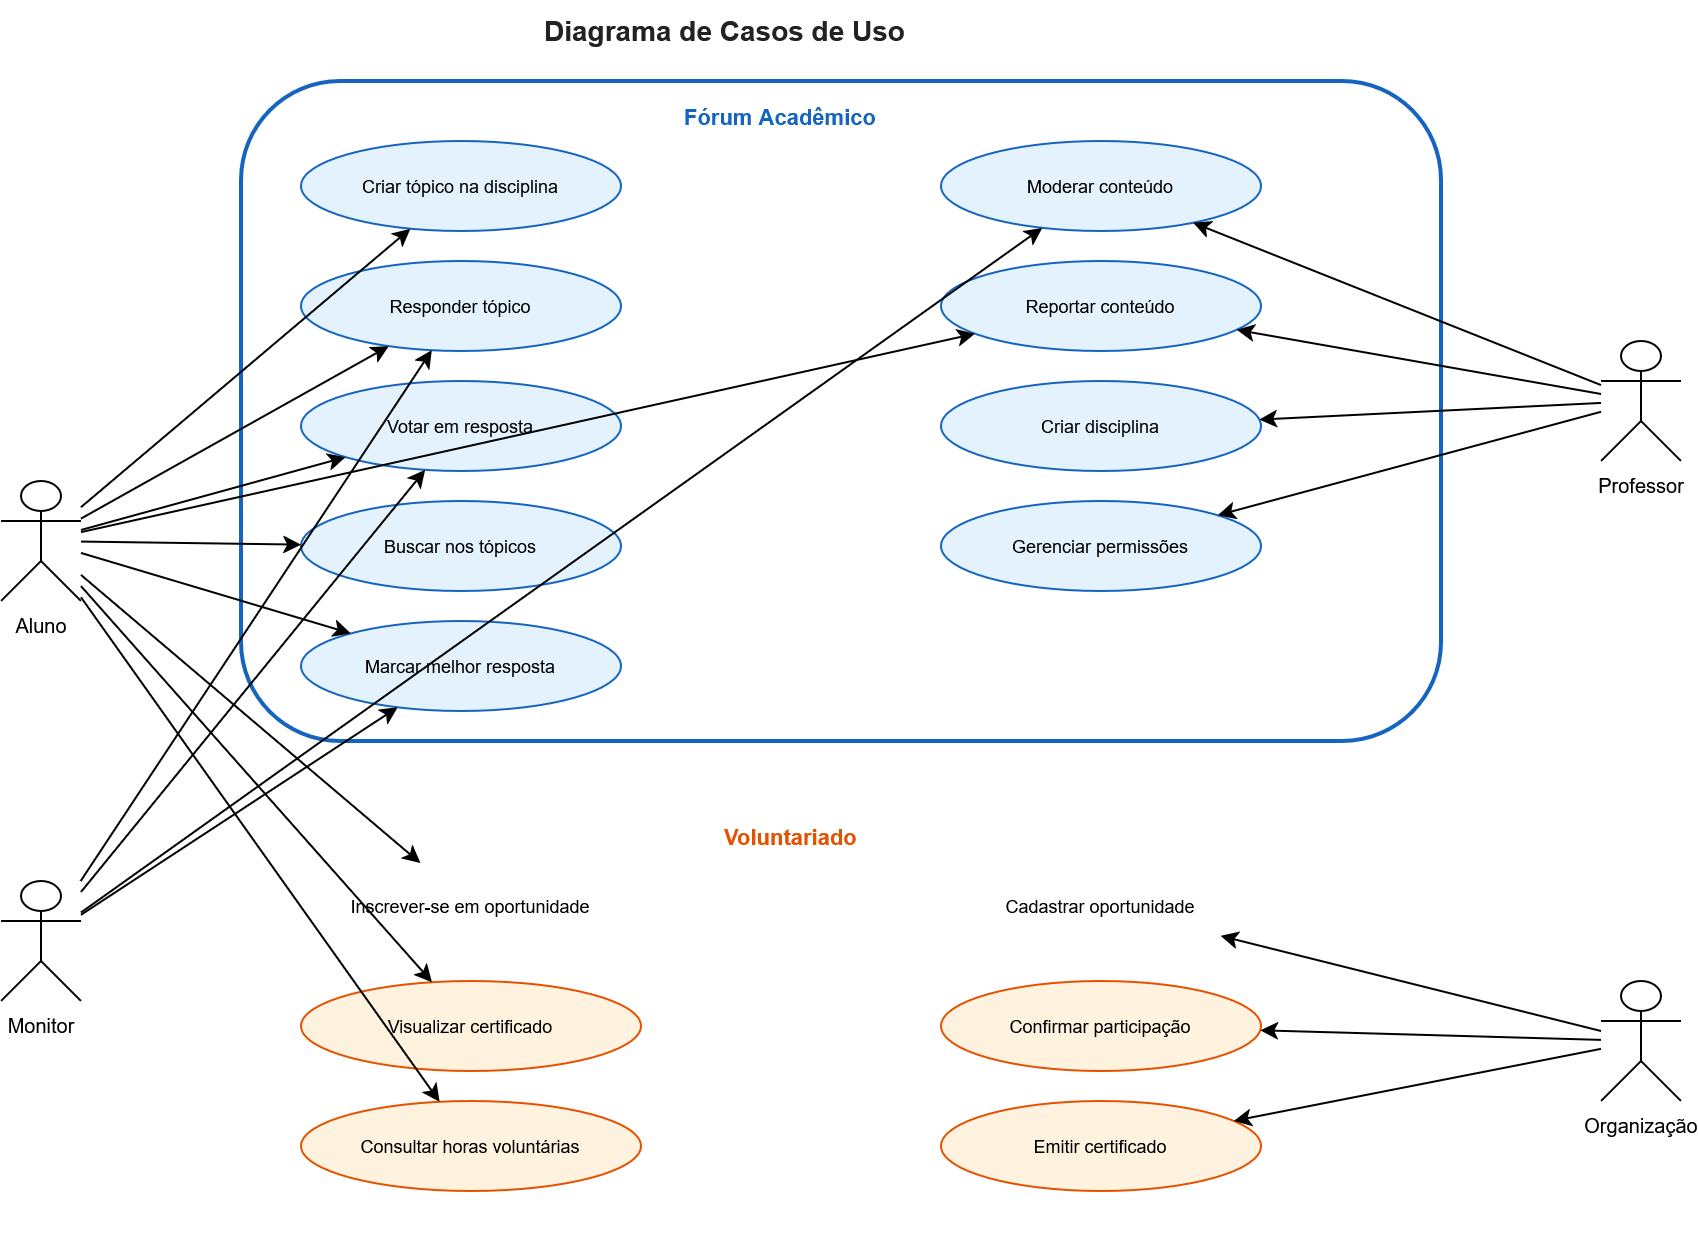
\includegraphics[width=\columnwidth]{figs/caso-de-uso.png}
\caption{Diagrama de casos de uso do sistema.}
\label{fig-casos-uso}
\textit{\scriptsize Fonte: Elaborado pela autora (2026).}
\end{figure}

A Figura \ref{fig-casos-uso} mostra o diagrama de casos de uso do sistema,
organizado em torno dos dois módulos centrais da plataforma: o fórum acadêmico e
o voluntariado. No módulo do fórum, o aluno pode criar tópicos, responder,
votar, fazer buscas e marcar a melhor resposta, enquanto o monitor e o professor
têm permissões a mais para moderar o conteúdo e cuidar das disciplinas. Já no
módulo de voluntariado, a organização cadastra as oportunidades e confirma a
participação dos alunos, enquanto o aluno se inscreve nas oportunidades, consulta
as horas que já tem registradas e visualiza os certificados que foram emitidos.

\subsection{Diagrama de Processos}

A Figura \ref{fig-processos} mostra o fluxo dos dois processos principais da
plataforma. No fórum, o aluno acessa a disciplina e faz uma busca nos tópicos
que já existem antes de criar um novo: caso ele encontre uma resposta que
resolva a sua dúvida, registra um voto e aquele conhecimento fica guardado para
as próximas consultas, e caso não encontre, cria um novo tópico que vai sendo
respondido por outros alunos ou monitores até que alguém marque a melhor
resposta e o tópico seja dado como resolvido. Já no voluntariado, a organização
cadastra a oportunidade, o aluno visualiza e se inscreve, participa da
atividade, a organização confirma a participação e o certificado é gerado
automaticamente, com as horas já registradas no perfil do aluno.

\begin{figure}[!ht]
\centering
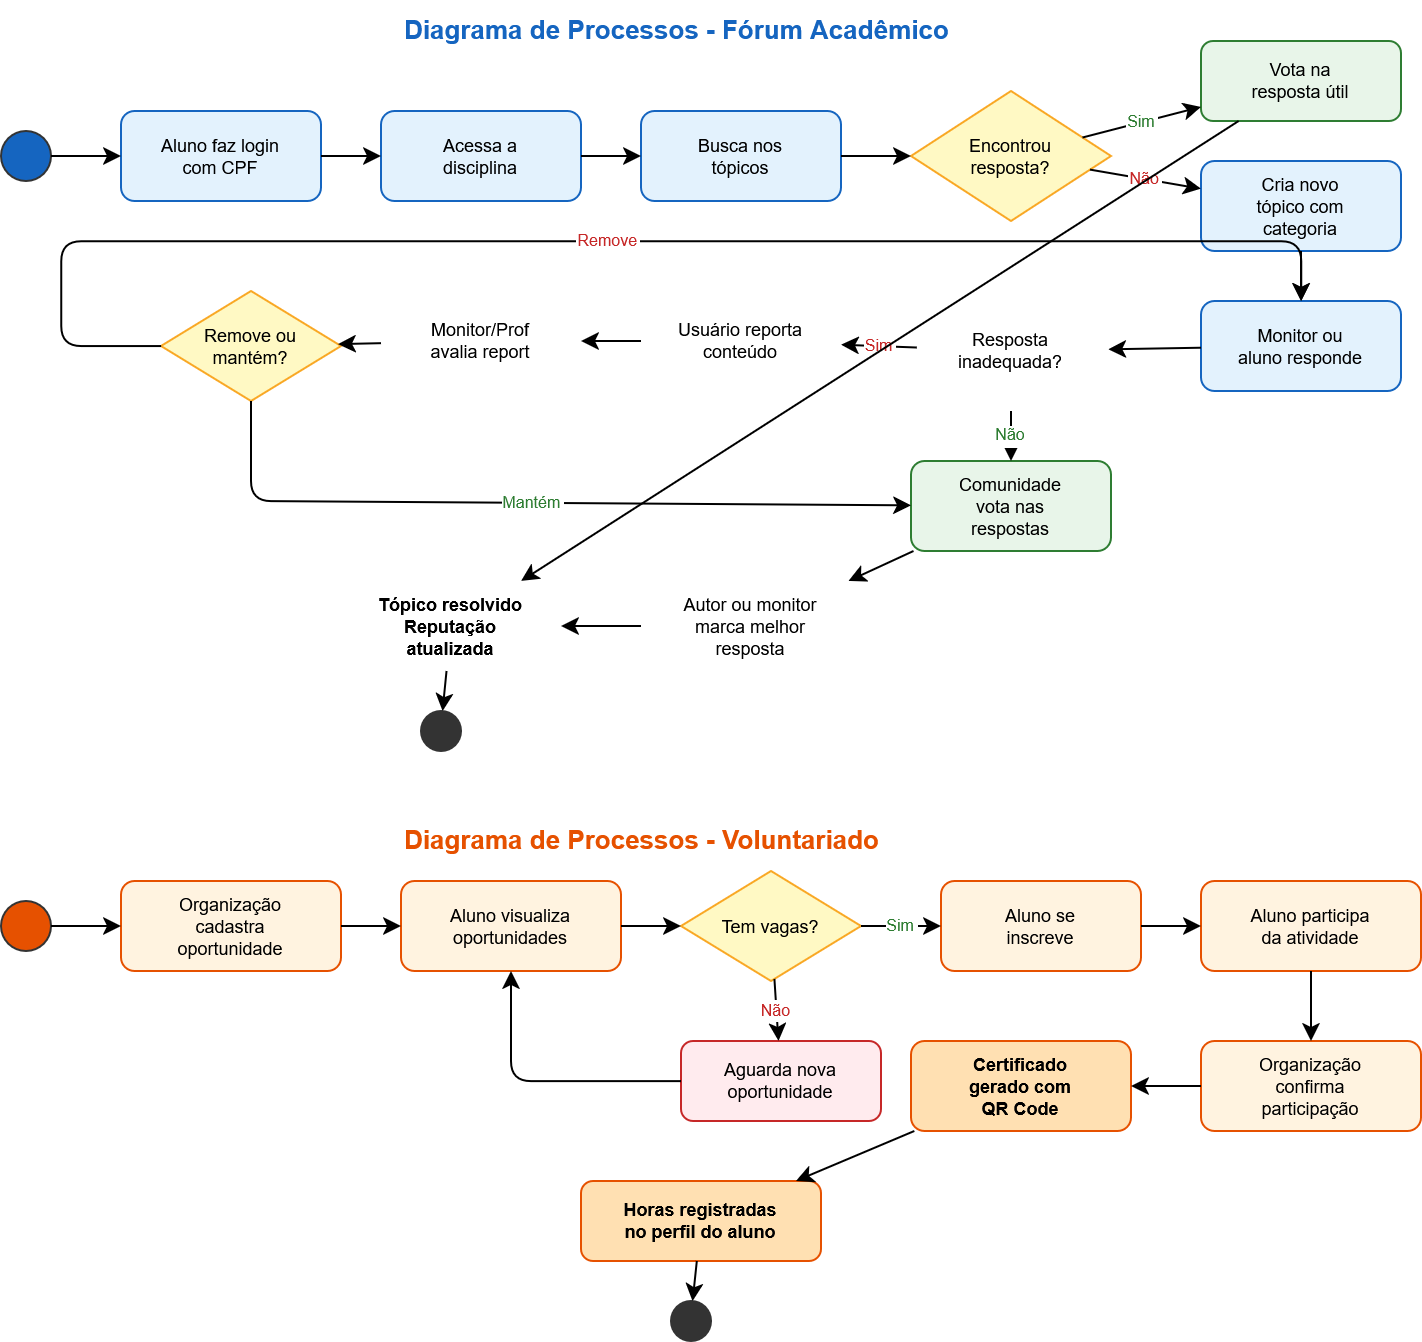
\includegraphics[width=0.5\textwidth]{figs/diagrama-processos.png}
\caption{Diagrama de processos do fórum acadêmico e do voluntariado.}
\label{fig-processos}
\textit{\scriptsize Fonte: Elaborado pela autora (2026).}
\end{figure}

\subsection{Diagrama de Implantação}

A Figura \ref{fig-implantacao} mostra como os componentes do sistema ficam
distribuídos em termos de infraestrutura. O usuário acessa a plataforma pelo
navegador, no qual o React.js roda localmente com a estilização do TailwindCSS.
As requisições passam por um servidor web Nginx, que entrega os arquivos
estáticos, como o HTML, o JavaScript e o CSS, e ainda funciona como proxy
reverso, mandando as chamadas da API REST para o servidor de aplicação, no qual
o Django roda junto com o Gunicorn (WSGI) para o tráfego HTTP comum, enquanto o
Daphne (ASGI) cuida das conexões WebSocket gerenciadas pelo Django Channels. O
Django se conecta ao PostgreSQL na porta 5432 para as operações com o banco e ao
Redis na porta 6379 para gerenciar os tokens JWT e as sessões ativas. As
credenciais de acesso ao banco e as outras configurações sensíveis ficam
guardadas em variáveis de ambiente, dentro de um arquivo \texttt{.env} que não
vai para o repositório do projeto, seguindo as boas práticas de segurança da
informação.
\begin{figure}[!ht]
\centering
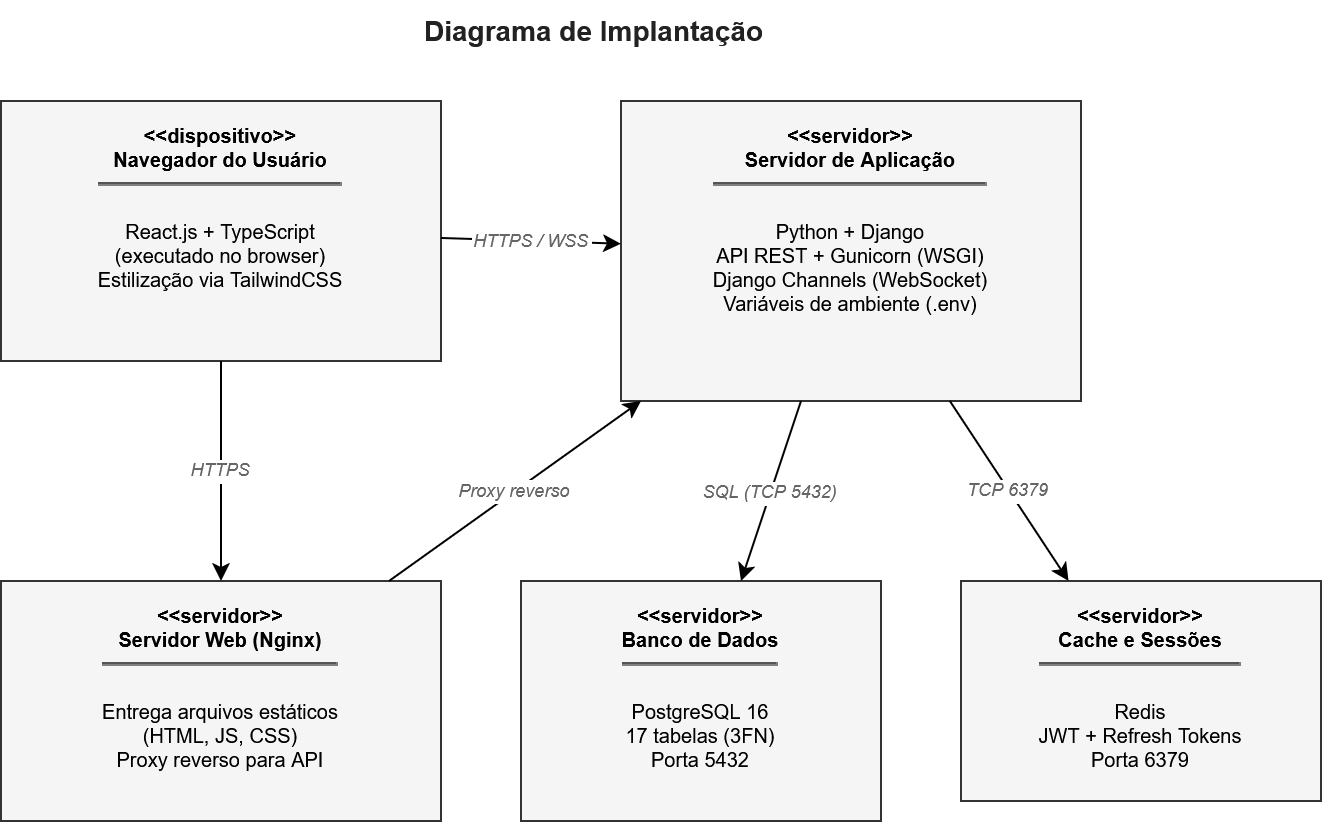
\includegraphics[width=0.50\textwidth]{figs/diagrama-implantacao.png}
\caption{Diagrama de implantação do sistema.}
\label{fig-implantacao}
\textit{\scriptsize Fonte: Elaborado pela autora (2026).}
\end{figure}
